\documentclass[11pt]{article}
\usepackage[utf8]{inputenc}
\usepackage{graphicx}
\usepackage{caption}
\usepackage{subcaption}
\usepackage{amsmath}
\usepackage{float}


\title{
	{Computer Vision 1 - Final Assignment\\
	 Bag-of-Words based Image Classification}
}
\author{
Selene Baez Santamaria (10985417) - Andrea Jemmett (11162929)}
\date{\today}

\begin{document}

\maketitle

\section{Implementation}
In this project we implement a system for image classification based of the Bag-of-Words approach. We train and test it with images provided by Caltech Vision Group concerning four categories \textit{Airplanes, Cars, Faces,} and \textit{Motorcycles}. 

\subsection{Feature Extraction and Description}
The first step in a Bag-of-Words image classification pipeline consists of
extracting features from a collection of images to successively use them to
build a visual vocabulary. To do this we extract SIFT descriptors from images
using \textit{VLFeat}. We define the function \texttt{sift\_descriptors.m}
that gets as input an image, the type of SIFT descriptors to extract (RGB, rgb
or opponent) and whether descriptors need to be extracted from keypoints or
densely. The function returns the extracted SIFT descriptors.

To extract SIFT features from color images we first convert the input image in
the requested color space. To do so we use a function that we created for Assignment 1, \texttt{convert\_color\_space.m}. However, some of the images provided are only grayscale and cannot be converted into a color space. In such cases we create a three channel image by copying the values into two extra layers and process the image as such. 

Next, for keypoint features we find a set of keypoints on the intensity image and use those frames to get local descriptors in each separate channel. This way if we detect $n$ keypoints, the normal SIFT descriptors will have size $128$, while for color SIFT we will have $128*3$. Therefore, the final descriptors matrix has size $n \times 128*3$.  For densely extracted features instead, we do not need to extract keypoints on the intensity image and features are extracted using a grid where the number of descriptors depends on the grid size.


\subsection{Building Visual Vocabulary}
Once we have a set of images represented as descriptors we use a clustering
technique to group together the most similar to each other until we reach a
stable set of $K$ clusters. We use \textit{Kmeans} through the use of the
function \texttt{vl\_kmeans} offered by \textit{VLFeat}. The clusters resulting from the operation become the set of words used in the vocabulary, so that $K$ controls the size of the vocabulary.


\subsection{Features Quantization}
Once we have a vocabulary of visual words we can transform an image as a
collection of visual words. To do this we created two functions:
\texttt{as\_bag.m} and \texttt{hist\_from\_bags.m}.

The former gets as input an image, the vocabulary and SIFT parameters like the
type (RGBSIFT, rgbSIFT and opponentSIFT) and if we want dense- or keypoint-based
descriptors. For each feature vector extracted (of size 384) we find the visual
word in the vocabulary that is the closest to the feature vector. We compute
their difference and then the norm of the resulting, assigning the visual word
in the vocabulary that has the lowest norm value.

The latter is responsible of converting a collection of images represented as
bags of visual words into normalized histograms of visual words count. For doing so, we count how many times a visual word appears in a bag and then normalize by dividing by the total number of words in the image. As a consequence our histograms contain only numbers in the range $[0, 1]$, which has proven to improve successive classification performance.


\subsection{Classification}
Now that we can represent an image as a frequency of words, we can use it as the input for a classification tool. Given that we have four categories, we create four binary classifiers so that each classifier outputs the probability of the image containing the specific object. The classifier model we use is a  Support Vector Machine (SVM), with the implementation provided by \textit{LIBSVM}.

In order to run a whole simulation the following commands must be run in Matlab:

\begin{enumerate}
	\item \textit{main}
	\item \textit{train}
	\item \textit{test}
	\item \textit{plots}
\end{enumerate}


\section{Evaluation}
Once the pipeline is complete we are able to explore the effect that different parameters have on the classification performance. In order to measure this performance we take the Average Precision (AP) per object class and the mean over four classes (mAP). 

\subsection{Sampling}
First we evaluate the difference between keypoints and dense sampling. For dense sampling we selected the following parameters $step-size = 30$ and $block-size = 6$ which leads to approximately 170 descriptors per image. 

The results are shown in the following table and visualized in Figure \ref{fig:sampling}.

\begin{center}
	\begin{tabular}{| c | c | c | c | c | c |}
		\hline
		\textbf{} & \textbf{Airplane} & \textbf{Cars} & \textbf{Faces} & \textbf{Motorbikes} & \textbf{mAP} \\ \hline
		\textbf{Keypoints} & 0.8463 & 0.8872 & 0.7344 & 0.9238 & 0.8480 \\ \hline
		\textbf{Dense} & 0.9362 & 0.8897 & 0.9552 & 0.8467 & 0.9069 \\ 
		\hline
	\end{tabular}
\end{center}

\begin{figure}[h]
	\centering
	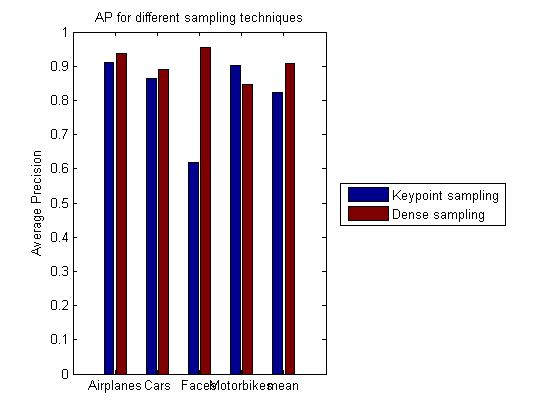
\includegraphics[width=.8\textwidth]{img/sampling.jpg}
	\caption{AP for different categories (airplanes, cars, faces and motorbikes) for keypoint and dense.}
	\label{fig:sampling}
\end{figure}

We note that dense sampling is generally more precise than keypoint sampling. A possible explanation is that dense sampling has spatial structure, which is important for most of the object classes implied in this assignment, especially for Faces as shown in the bar graph.

Here on, we perform all runs with keypoint sampling. 

\subsection{Color descriptors}
Secondly, we change the descriptor type to rgbSIFT or opponentSIFT. Compared to regular RGBSIFT, the results are shown in the following table and visualized in Figure \ref{fig:color_descriptors}.

\begin{center}
	\begin{tabular}{| c | c | c | c | c | c |}
		\hline
		\textbf{} & \textbf{Airplane} & \textbf{Cars} & \textbf{Faces} & \textbf{Motorbikes} & \textbf{mAP} \\ \hline
		\textbf{RGB} & 0.8463 & 0.8872 & 0.7344 & 0.9238 & 0.8480 \\ \hline
		\textbf{rgb} & 0.9728 & 0.8969 & 0.8278 & 0.7775 & 0.8687 \\ \hline
		\textbf{opp} & 0.9570 & 0.9218 & 0.9392 & 0.8438 & 0.9155 \\ 
		\hline
	\end{tabular}
\end{center}

We note that rgb generally performs better than RGB, except for the Motobikes class. Since we know that RGB is not invariant to shadows and shading, but rgb and opponent colors are, a possible explanation for RGB's higher performance is the fact that most Motorbikes have small pieces put together with empty spaces between them, which leads to images rich in shadows. 

Additionally, our results agree with previous research which has shown that the opponent color descriptors outperform other color spaces. 

\begin{figure}[h]
	\centering
	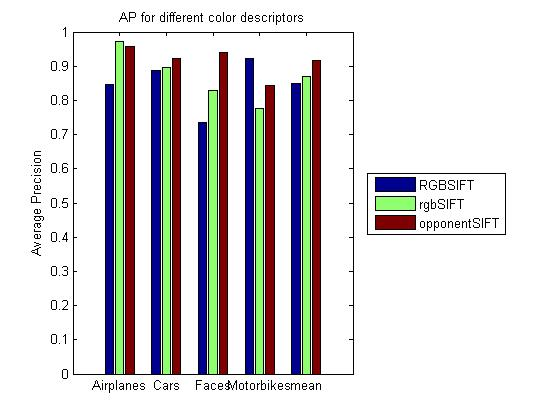
\includegraphics[width=.8\textwidth]{img/color_descriptors.jpg}
	\caption{AP for different categories (airplanes, cars, faces and motorbikes) for three different color descriptor: RGB-SIFT, rgb-SIFT and opponent-SIFT.}
	\label{fig:color_descriptors}
\end{figure}

Here on, we perform all runs with RGB-SIFT unless otherwise stated.

%\subsection{PCA-SIFT}

\subsection{Vocabulary size}
Next, we increase the length of the vocabulary to see if this increases the performance. The results are shown in the following table, plotted in Figure \ref{fig:voc_size_plot}. Due to computational power limitations, only values of $voc-size = 400$ , $voc-size = 1600$ and $voc-size = 4000$ were tested.

\begin{center}
	\begin{tabular}{| c | c | c | c | c | c |}
		\hline
		\textbf{} & \textbf{Airplane} & \textbf{Cars} & \textbf{Faces} & \textbf{Motorbikes} & \textbf{mAP} \\ \hline
		\textbf{400 words} & 0.8463 & 0.8872 & 0.7344 & 0.9238 & 0.8480 \\ \hline
		\textbf{1600 words} & 0.9399 & 0.8744 & 0.6194 & 0.8895 & 0.8308 \\ \hline
		\textbf{4000 words} & 0.9464 & 0.9076 & 0.7766 & 0.9303 & 0.8902 \\ 
		\hline
	\end{tabular}
\end{center}

\begin{figure}[h]
	\centering
	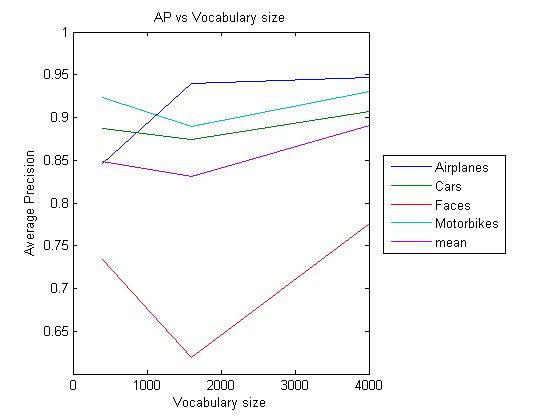
\includegraphics[width=.8\textwidth]{img/voc_size_plot.jpg}
	\caption{AP for different categories (airplanes, cars, faces and motorbikes) as the vocabulary size increases.}
	\label{fig:voc_size_plot}
\end{figure}

This time we note that generally increasing the length of our vocabulary from 400 to 1600 has a negative effect on performance. Although it may benefit some specific classes, like the Airplanes class AP increases by 10\% in our case, some other classes suffer the opposite effect and decrease their accuracy by the same factor, like the Faces class AP decreasing around the same 10\%. This may be interpret as saying that airplanes benefit from a larger variety of features to uniquely identify them, while faces find this distinction disturbing.

However, increasing from 1600 to 4000 has a steady beneficial effect over all classes.

Here on, we perform all runs with vocabulary size $voc_size = 400$.

\subsection{Training samples}
This time we experiment with different values for the training set. Here we determine the number $n$ of positive examples that will be fed to the SVM, and assume there are three times as many negative examples in the training set, meaning $3*n$. This leads to a total training set of $4*n$ samples. 

The results for $n = 50$ and $n=200$ are summarized in the following table and plotted in Figure \ref{fig:training_size_plot}.

\begin{center}
	\begin{tabular}{| c | c | c | c | c | c |}
		\hline
		\textbf{} & \textbf{Airplane} & \textbf{Cars} & \textbf{Faces} & \textbf{Motorbikes} & \textbf{mAP} \\ \hline
		\textbf{50 samples per class} & 0.9121 & 0.8640 & 0.6185 & 0.9016 & 0.8241 \\ \hline
		\textbf{200 samples per class} & 0.8463 & 0.8872 & 0.7344 & 0.9238 & 0.8480 \\ \hline
		\hline
	\end{tabular}
\end{center}

\begin{figure}[h]
	\centering
	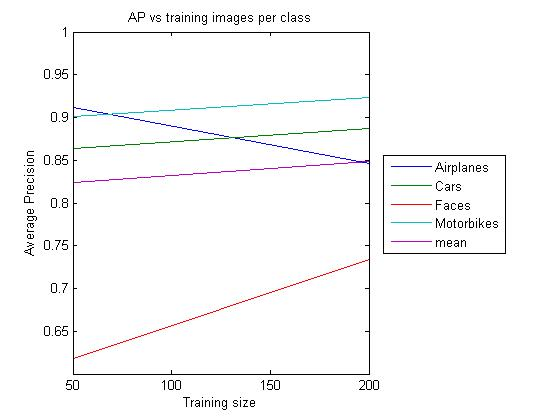
\includegraphics[width=.8\textwidth]{img/training_size_plot.jpg}
	\caption{AP for different categories (airplanes, cars, faces and motorbikes) as the number of training images per class increases.}
	\label{fig:training_size_plot}
\end{figure}

We note that the effect is inverse to the vocabulary size effect. Again, the effect varies between specific object classes, Airplanes and Faces. However, this time Airplanes suffer from a larger training sample while Faces benefit from it. 

Furthermore, we conclude that as the training set increases in size, mean accuracy increases as expected. Given this information, we can compare the effect of training size compared to color descriptors on AP.

The results are shown in the following table and visualized in Figure \ref{fig:training_size_color}.

\begin{center}
	\begin{tabular}{| c | c | c | c |}
		\hline
		\textbf{} & \textbf{RGB} & \textbf{rgb} & \textbf{opponent} \\ \hline
		\textbf{50 samples per class} & 0.8241 & 0.8552 & 0.8826 \\ \hline
		\textbf{200 samples per class} & 0.8480 & 0.8687 & 0.9155 \\ \hline
		\hline
	\end{tabular}
\end{center}
. 
\begin{figure}[h]
	\centering
	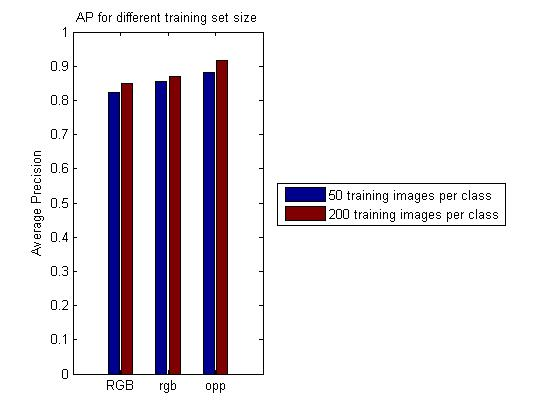
\includegraphics[width=.8\textwidth]{img/training_size_color_descriptor.jpg}
	\caption{mAP for three different color descriptors (RGB-SIFT, rgb-SIFT and opponent-SIFT) as the number of training images per class increases.}
	\label{fig:training_size_color}
\end{figure}

This bar graph confirms our two previous conclusions. Firstly, that the color descriptors behaviour (rgbSIFT outperforms RGBSIFT, and opponentSIFt outperforms the previous two) is stable accross different training set sizes. Secondly, a larger training set benefits the AP, even across different color spaces. 

Here on, we perform all runs with $n = 50$. 

\subsection{SVM Kernel}
Finally, we investigate the performance for various types of kernels in the SVM. The available options in \textit{LIBSVM} are \textit{Linear, RBF, Polynomial} and \textit{Sigmoid}. 

The results are shown in the following table and visualized in Figure \ref{fig:svm_kernel}. 

\begin{center}
	\begin{tabular}{| c | c | c | c | c | c |}
		\hline
		\textbf{} & \textbf{Airplane} & \textbf{Cars} & \textbf{Faces} & \textbf{Motorbikes} & \textbf{mAP} \\ \hline
		\textbf{Linear} & 0.8463 & 0.8872 & 0.7344 & 0.9238 & 0.8480 \\ \hline
		\textbf{RBF} & 0.8732 & 0.7919 & 0.6892 & 0.8486 & 0.8007 \\ \hline
		\textbf{Polynomial} & 0.6967 & 0.6202 & 0.5176 & 0.6342 & 0.6172 \\ \hline
		\textbf{Sigmoid} & 0.8650 & 0.7982 & 0.6780 & 0.8459 & 0.7968 \\ 
		\hline
	\end{tabular}
\end{center}

\begin{figure}[h]
	\centering
	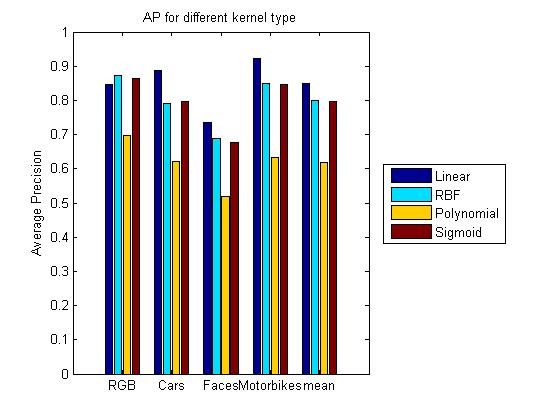
\includegraphics[width=.8\textwidth]{img/svm_kernel.jpg}
	\caption{mAP for different categories (airplanes, cars, faces and motorbikes) as number of training examples increases.}
	\label{fig:svm_kernel}
\end{figure}

We note that the best mean performance is a consequence of Linear kernels. Our reasoning for explaining such an effect is the data are already high dimensional, so kernels that transform the data into even higher dimensional spaces are non-beneficial.

\section{Reflection}
While working on this project we noticed that on the one side, K-means clustering consumes large computational resources. Because the complexity of K-means (for a problem with fixed clusters $k$, $n$ data samples of dimension $d$) can be written as $O(n^{dk+1}\log{n})$, it is easy to note how for this problem $K=4000$ clusters with $d=128*3$ and $n=4*200$ the complexity gets important. For this reason, we had to truncate many runs that took over 2 hours to evaluate on powerful machines. 

On the other side, the SVM implementation provided by LIBSVM is notably fast which allowed us to train models in a few minutes. Yet, the histogram construction represented yet another bottleneck in complexity since it compares all words in the image to all words in the vocabulary. It is again easy to see how this rapidly increases by having a larger vocabulary.


\end{document}

